\begin{question}
\noindent Shape $Q$ is shown on the grid below. Point $O$ is marked as a centre of enlargement.

\begin{center}
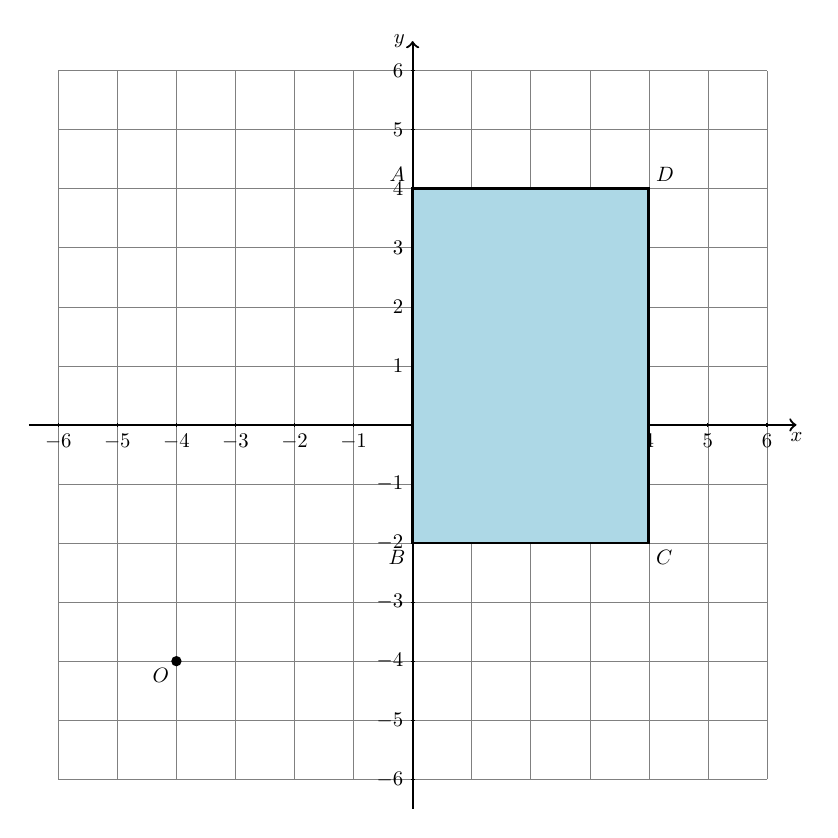
\begin{tikzpicture}[scale=0.75, transform shape]
    \definecolor{borderColour}{HTML}{000000}
    \definecolor{fillColourQ}{HTML}{ADD8E6}

    \def\axisLimit{6}

    % Draw grid
    \draw[step=1cm,gray,very thin] (-\axisLimit,-\axisLimit) grid (\axisLimit,\axisLimit);

    % Draw axes
    \draw[thick,->] (-\axisLimit-0.5,0) -- (\axisLimit+0.5,0) node[anchor=north] {$x$};
    \draw[thick,->] (0,-\axisLimit-0.5) -- (0,\axisLimit+0.5) node[anchor=east] {$y$};

    % Label x-axis and y-axis
    \foreach \x in {-\axisLimit,...,-1,1,2,...,\axisLimit}
        \draw (\x cm,1pt) -- (\x cm,-1pt) node[anchor=north] {$\x$};
    \foreach \y in {-\axisLimit,...,-1,1,2,...,\axisLimit}
        \draw (1pt,\y cm) -- (-1pt,\y cm) node[anchor=east] {$\y$};

    % Centre of enlargement O
    \coordinate (O) at (-4,-4);
    \fill[black] (O) circle (2.5pt);
    \node[below left] at (O) {$O$};

    % Define vertices of Q
    \coordinate (A) at (0,4);
    \coordinate (B) at (0,-2);
    \coordinate (C) at (4,-2);
    \coordinate (D) at (4,4);

    % Draw Q
    \draw[fill=fillColourQ, draw=borderColour, line width=1pt] (A) -- (B) -- (C) -- (D) -- cycle;
    \node[above left] at (A) {$A$};
    \node[below left] at (B) {$B$};
    \node[below right] at (C) {$C$};
    \node[above right] at (D) {$D$};

\end{tikzpicture}
\end{center}

\noindent Enlarge shape $Q$ by scale factor $\dfrac{1}{2}$, centre of enlargement $O(-4,-4)$.

\begin{enumerate}
    \item[(a)] Work out the coordinates of the image of each vertex of shape $Q$.

    \vspace{5cm}
    \answerplain{2}

    \item[(b)] On the grid above, draw the enlarged shape $Q'$.

    \vspace{1cm}
    \answermarks{1}
\end{enumerate}
\end{question}
